%\documentclass[letterpaper, 10pt]{sigcomm-alternate}

\documentclass[peerreview, a4paper, 7pt]{IEEEtran}
%\documentclass[a4paper, 10pt]{IEEEtran}
%\documentclass{scrreprt}
\usepackage{times}
\usepackage{alltt}
\usepackage{graphicx}
\usepackage{alltt}
\usepackage{colortbl}
\usepackage[dvipsnames]{xcolor}

%\usepackage{color}
% \usepackage{caption2}
%\usepackage{subfigure}
%\usepackage{graphicx}
%\usepackage{colortbl}
%\usepackage[dvipsnames]{xcolor}
% \usepackage{ulem}

\usepackage{hyperref}

\pagenumbering{arabic}


%\ifx\pdfoutput\undefined
%\usepackage[pdfpagemode=none, pdfstartview=FitH, colorlinks=true, urlcolor=black, linkcolor=black, citecolor=black]{hyperref}
%\else
%\usepackage[pdftex, pdfpagemode=none, pdfstartview=FitH, colorlinks=true, urlcolor=black, linkcolor=black, citecolor=black, pdftex]{hyperref}
%\fi

\ifx\HCode\UnDef\else\hypersetup{tex4ht}\fi

%% Editorial work
% \newcommand{\purge}[1]{\textcolor{red}{\sout{#1}}}
% \newcommand{\add}[1]{\textcolor{blue}{#1}}

%%% End of editorial work.


 
\renewcommand{\em}[1]{\textit{#1}}
\begin{document}

\title{Software and Firmware Updates with the OMA LWM2M Protocol}

\author{\authorblockN{Hannes Tschofenig\authorrefmark{1}\\}
\authorblockA{\authorrefmark{3}ARM Limited, 
Email: hannes.tschofenig@arm.com\\}
\thanks{\textsc{Position paper for the 'Internet of Things Software Update Workshop (IoTSU)'~\cite{IOTSU}, 13$^{th}$ and 14$^{th}$ June 2016, Dublin, Ireland.} The content of this document describes the views of the author.}
}

\date{\today}

\maketitle


\section{Abstract}


The Lightweight Machine-to-Machine (LWM2M)~\cite{lwm2m} protocol has been developed by the Open Mobile Alliance (OMA) to provide a number of device management functions, including software and firmware updates. With the mbed client and the mbed Connector ARM has implemented LWM2M and offers it to developers. This position paper describes what functionality has been standardized in LWM2M for software and firmware updates and what open issues exist. 

\section{LWM2M Overview}
\label{lwm2m}

The high-level architecture of LWM2M is shown in Figure~\ref{lwm2m-architecture-figure} where the LWM2M client, running on an IoT device, interacts with a LWM2M server. With LWM2M v1.0 the use of CoAP over UDP as well as CoAP over SMS are supported. For communication security the use of DTLS is assumed. Various RESTful APIs (i.e., interfaces) are offered to allow communication of structured data. The data is organized in form of objects, that contain resources. The detailed structure of the data model has been subject to separate position paper published in the IoT Semantic Interoperability Workshop 2016, see~\{cite{ipso-iotsi-paper}. 

\begin{figure}[!htbp]
 \centering
 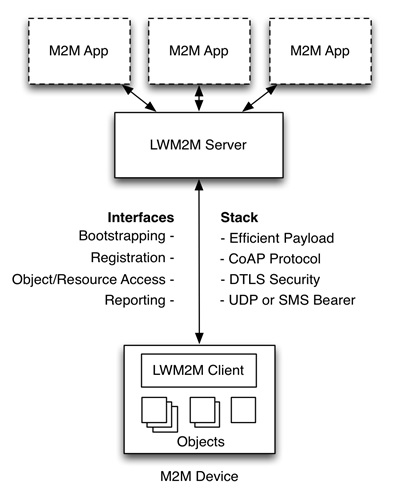
\includegraphics[scale=0.50]{lwm2m-architecture.jpg}
 \caption{LWM2M Architecture.}
 \label{lwm2m-architecture-figure}
\end{figure}

A number of objects have been standardized already to allow the exchange of data between an IoT device and the server-side infrastructure. This communication is bi-directional and allows the server to obtain, for example, sensor readings but to also control actuators. The same object model is used for the interactions. A full list of the already standardized objects can be found at a registry maintained by the OMA~\cite{OMNA}. This registry contains a firmware object as well as a software management object. The functionality of the two is described in the subsections below.

\subsection{Firmware Object} 
The object definition of the firmware object can be found at~\cite{firmware-object}. It includes a number of resources, namely 
\begin{enumerate}
\item The firmware package itself or a URI pointing to it. The idea of using a URI is to allow a server to instruct a client to download the firmware from another source. 
\item Various resources to expose the protocol interaction and the result of the firmware update operation. For example, the Update Result resource allows a LWM2M client to expose information about the reason for a failed software update or that the update has been performed successfully. 
\end{enumerate}

The process for providing a firmware to a device is supposed to happen in two stages, namely the download of the firmware image and subsequently the executation of the update. An update can only be executed when the device has successfully downloaded the firmware image (and presumably took the necessary verification steps) and has transitioned into the 'Downloaded' state. 

The object definition indicates that only a single firmware object can be present on a device. Furthermore, there is no meta-data in the object definition about the content of the firmware package. 

\subsection{Software Management Object}
Since the firmware object was seen as too basic an extended version, called software management object, was developed. The object definition of the software management object is not included in the main LWM2M specification but has instead been published as a separate specification~\cite{SwMgmt}. Two objects have been defined, namely the Software Component object (with object id 14) and the Sofware Management object (with object id 9). 

The added functionality provided by these two objects aims to focus on devices where multiple software packages are installed. Similiarly to the firwmare update procedure the server can push a software package or a URI to a software package. To support the download of packages by the client using the provided URI the server may also provision as username/password to the client, if authentication is needed to download the software package. As a difference to the firmware update procedure it is also necessary to activate software after it has been installed. Furthemore, deactivating and removing a software package is also supported. 

The Software Management object furthermore defines basic meta-data about the name and the version of the package and contains one or multiple links to Software Component objects. Figure~\ref{software-management-figure} shows the relationship between the two objects graphically. 

\begin{figure}[!htbp]
 \centering
 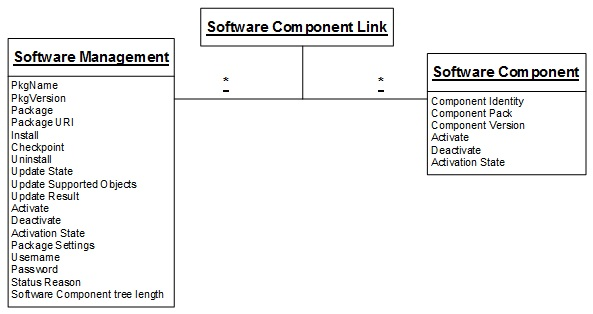
\includegraphics[scale=0.50]{software-management.jpg}
 \caption{Software Management.}
 \label{software-management-figure}
\end{figure}

As shown, the software management object may contain of one or more software components. In addition to the multiple software components a device may also have multiple software management objects. 

\section{What are we trying to standardize?}
\label{what}

The OMA work on software and firmware updates, as two independent solutions, hints to the fuzzy definition of Internet of Things. IoT devices, in ARM jargon, may be devices that run Cortex A class processors and are therefore able to general purpose operating systems, such as Arch Linux, since they are equipped with a memory management unit, use more powerful processors, and also have more RAM and flash memory. Devices with such operating systems have, for a long time, been using sophisticated software update mechanisms (such as Pacman). Software has also been provided by different developers and thanks to the isolation techniques offered by the hardware and modern operating systems, a failure in one software typically does not impact other software components (from a security point of view). Often software update on these devices allow updates to be obtained from various sources. 

\textsc{Question}: Do we need additional software update standards for these A-class devices?

To make the question more complicated, many A-class type processors offer a hardware security features called Trusted Execution Environments (TEEs)~\cite{TEE}. These TEEs provide a separation between the full blown, general purpose operating system and a real-time operating system. The two sides are often referred as normal world and secure world. The purpose of the separation is to place security sensitive components in the smaller, better audited, and more tightly controlled real-time operating system and to use hardware features to control the transition between the two worlds. Software/firmware updates for the secure world are often very different, technically and operationally, from the update mechanism used in the normal world.

\textsc{Question}: Is there a need for a software/firmware update mechanism used in the secure world on such A-class alike devices? 

Moving from the Cortex A-class devices to the more constrained Cortex M-class devices a different software development pratice has been established. While software has gotten more and more complex with the desire to connect to various Internet services a single firmware image is in the end uploaded to the M-class IoT device. This image typically contains software libraries from various sources and may even contain binary imagines that have been provided by silicon manufacturers. This means that in some cases the developer may not have access to the full source code but instead has to link a binary to his or her code\footnote{An example of this approach can be seen with the Bluetooth Low Energy (BLE) microcontrollers offered by Nordic Semiconductor, such as the Nordic nRF51-DK~\cite{nRF51-DK}. Nordic thereby offers the BLE protocol stacks as so-called SoftDevices for download. SoftDevices are pre-compiled, pre-linked binary files, which subsequently need to linked to the actual application code (such as a BLE peripheral providing the features of a heartrate monitor.)}.

While some companies have been experimenting with the Java Virtual Machines, or similiar sandboxing techniques to allow downloading software components from different sources these efforts typically face challenges with the nature of the M-class devices. These devices are supposed to be cheap, purpose built, energy efficient and equipped with limited resources (RAM, flash, etc.).  

\textsc{Question}: What are the minimum requirements for firmware updates for such M-class devices? What components need to be standardized to make it easier for developers to improve security of their IoT software?

Security has been an important consideration for all Internet connected devices and TEEs have been introduced to A-class devices (with ARM TrustZone) many years ago already. In November 2015 ARM has also made a technology launch of TrustZone for v8-M~\cite{Trustzone} and thereby completed the v8 architecture for application (A), real-time (R), and microcontroller (M) devices. It remains to be seen whether the developer experience for devices using TrustZone for v8-M and v8-A will be similar or very different. Other hardware security features may impose a certain deployment or certain developer model.

\textsc{Question}: How do hardware security features for embedded devices impact firmware update mechanisms?

\section{Open Issues with LWM2M}
\label{open-issues}
The introduction to LWM2M also indicates what functionality has not been standardized and there may be good reasons for leaving certain functionality either out of scope or subject to proprietary implementations. The following subsections highlight a few of the identified open issues. 

\subsection{Choice of Transport and Fragmentation}

Firmware updates may potentially be large (in the range of > 100 KiB for a Cortex M-based device). Although the transport of software and firmware updates has been standardized with LWM2M the use of CoAP, which runs on top of UDP, quickly leads to problems. First, UDP has a maximum size limit of ~64 KiB. Second, transmitting UDP messages that are larger than the path MTU size leads to fragmentation of these messages at the lower layers, typically IP. It may also lead to fragmentation at the adaptation layer. 

It turns out that CoAP over TCP as well as the blockwise transfer developed for CoAP more recently in the IETF CoRE working group can help to mitigate these problems. Unfortunately, the LWM2M v1.0 does not support these newer CoAP extensions. As a consequence, software/firmware updates with file sizes larger than ~64 KiB are not supported. Furthemore, the performance of any software/firmware update using CoAP alone (without utilizing these extensions) over low power radio technologies (such as IEEE 802.16.4, or the recently developed low power wide area networks) will be significiantly degrated due to the interplay between packet loss and the fragmentation behavior at the IP or the adaptation layer.

When firmware images are distributed to a large number of devices the caching capabilities of CoAP (and other protocols) may turn out to be useful, including multicast support, but are not discussed in the LWM2M specification.

Ideally, a firmware distribution mechanism should offer flexible transport to allow it to be used over a number of different technologies. Some of these radio technologies are lossy, require re-transmission of a subset of the transmitted data. Efficiency of the firmware distribution is important since a firmware update of a device running on a coin-cell battery can easily drain half of the battery capacity. 

\subsection{Meta-Data}

The LWM2M firmware object contains no meta-data about the firmware image itself and the Software Management object only contains a minimal amount of meta-data. Quite natually, the question arises what type of meta-data needs to be standardized as part of the data model. For example, the firmware object is only available as a single instance and this raises the question about the possibile implications for devices that have multiple microcontrollers, which will need independent updates. While this questions appears to be an hardware/software implementation design detail it does, however, have an impact on the data model. Would be it useful to capture the details of the internals of an IoT device to be able to communicate what microcontroller needs to be updated or is this a detail only the developer of the hardware needs to care about? 

Firmware images come in different formats, as Portable Executable (PE) and Executable and Linking Format (ELF), they may be compressed or come in form of diffs, they may consist of a single file or combined into multiple files. While it is certainly helpful to indicate the content type of the payloads being communicated is it useful for developers to settle on one or a few popular formats and compression techniques?

\subsection{Application Layer Security}

Protecting the transmission of software and firmware updates via DTLS is offered by LWM2M and communication layer security is definitely a viable option for protecting these sensitive payloads in flight, as well as to authenticate and authorizate the endpoints. When firmware images are cached in other locations (e.g., distributed to other servers, cached by proxies, used in a store-and-forward fashion) it maybe necessary to offer application layer security protection (e.g., message authentication codes, digital signatures, and potentially confidentiality protection) either as a replacement for communication security or in addition. Regarding serialization formats a number of choices do exist in the meanwhile, such as ASN.1/CMS, JSON/JOSE, and CBOR/COSE. While they are all fairly similar in functionality there are still suttle differences due to the history behind each of these efforts. What technique is most favorable by industry players? 

Since all these mechanisms are very flexible, different types of credentials are supported (e.g., symmetric keys, raw public keys, X.509 certs), with a varity of different cryptographic algorithms. Is there some profiling to increase interoperability and at the same time keep the code size as well as memory footprint to an acceptable level? To verify these protected payloads (and also for the use of communication security) the device needs to be provisioned with trust anchors, or other keying material to allow verification. These types of credentials may be used to force a certain deployment choice.

\section{Summary}
This document starts with an overview of the functionality provided by LWM2M in Section~\ref{lwm2m}. Section~\ref{what} then raises the question about where additional standardization work is needed. The answer will depend on the type of IoT device being dealt with and the level of interoperability the community desires. Finally, a couple of open issues are identified in the context of the LWM2M firmware/software update mechanism. 

By reaching out to the wider Internet community we hope to get more input on the currently deployed software/firmware update procedures. The most important building blocks and the best current practices should be standardized. These could serve as a valuable toolbox for developers trying to bring IoT devices faster to the market.

Besides the more technical aspects raised in the write-up above, there have been various concerns expressed by the Federal Trade Commission (FTC)~\cite{FTC} as well as by the Article 29 Working Party of the European Commission~\cite{Article29WP}. The concerns range from how end users should grant permissions for software updates (while on the other hand updating software as quickly as possible) to questions like 'Should modern refrigerators have a shelf-life, much like the food contained within?'~\cite{ShelfLife}. While these questions are important and need to be answered by the wider community the author believes that the IOTSU workshop~\cite{IOTSU} will less likely to make progress on answering these questions.  

\bibliographystyle{IEEEtran}
% \bibliographystyle{acmtrans}
\bibliography{paper}


\end{document}

